\chapter{The RISC-V processor}
    We are finally at a point where we can start building the RISC-V CPU in SME. At the start of this project I followed the approach described in chapter 4 of the RISC-V book \cite{riscVbook}, but when a functioning CPU was made I quickly came to the realization that the version described in the book was quite inadequate. It only supported a handful instructions, which is not enough to run any but the simplest of programs. 
    
    Therefore I had to sit down and design a version with the requirement of supporting all 49 basic RISC-V instructions. This design of course took foundation in the book version, with improvements from the lessons learned from the first implementation.
    
    Throughout this chapter we will go through the new design, which can be found here\footnote{\url{https://github.com/DanielRamyar/Master_Thesis/tree/master/SME_Implementations/SingleCycleRISCV2}}.

\section{Single Cycle RISC-V Units}
    In this section we will explain the function of each of the 14 units, used in the implementation of the CPU. This design is single cycle, meaning that only one instruction is executed per clock cycle. 

    \subsection{Program Counter}
        The \textit{program counter}, PC for short, keeps track of where in the program we are located and is a fairly simple unit. It can we thought of a single register, which holds the address of the current instruction.
        
        To implement the PC unit we create a clocked SME process. It needs to be clocked, meaning the unit will activate on a rising clock edge, as it will part of a closed loop circuit, when we later connect the units. If no unit is clocked in a closed loop, there is no way of knowing, where to begin sending signals. Therefore the PC was chosen to be clocked, as it seemed like the most logical place to start the signal propagation.
        
        The PC process contains a single \texttt{ulong} integer, which will hold the instruction address. The input bus contains the address of the next instruction and the output bus the current. You may ask how the process outputs the current address, when it reads the next address first. Remember that the process is clocked, so when it reads the next address input, it will actually contain the address calculated in the previous clock cycle, as the bus hasn't been updated yet. This would then be the correct address in the current clock cycle.
        
        The PC process has been illustrated in Figure \ref{fig:PC} and a code segment is shown in Listing \ref{PCSME}. 
        
        
        
        \begin{figure}[h!]
            \centering
            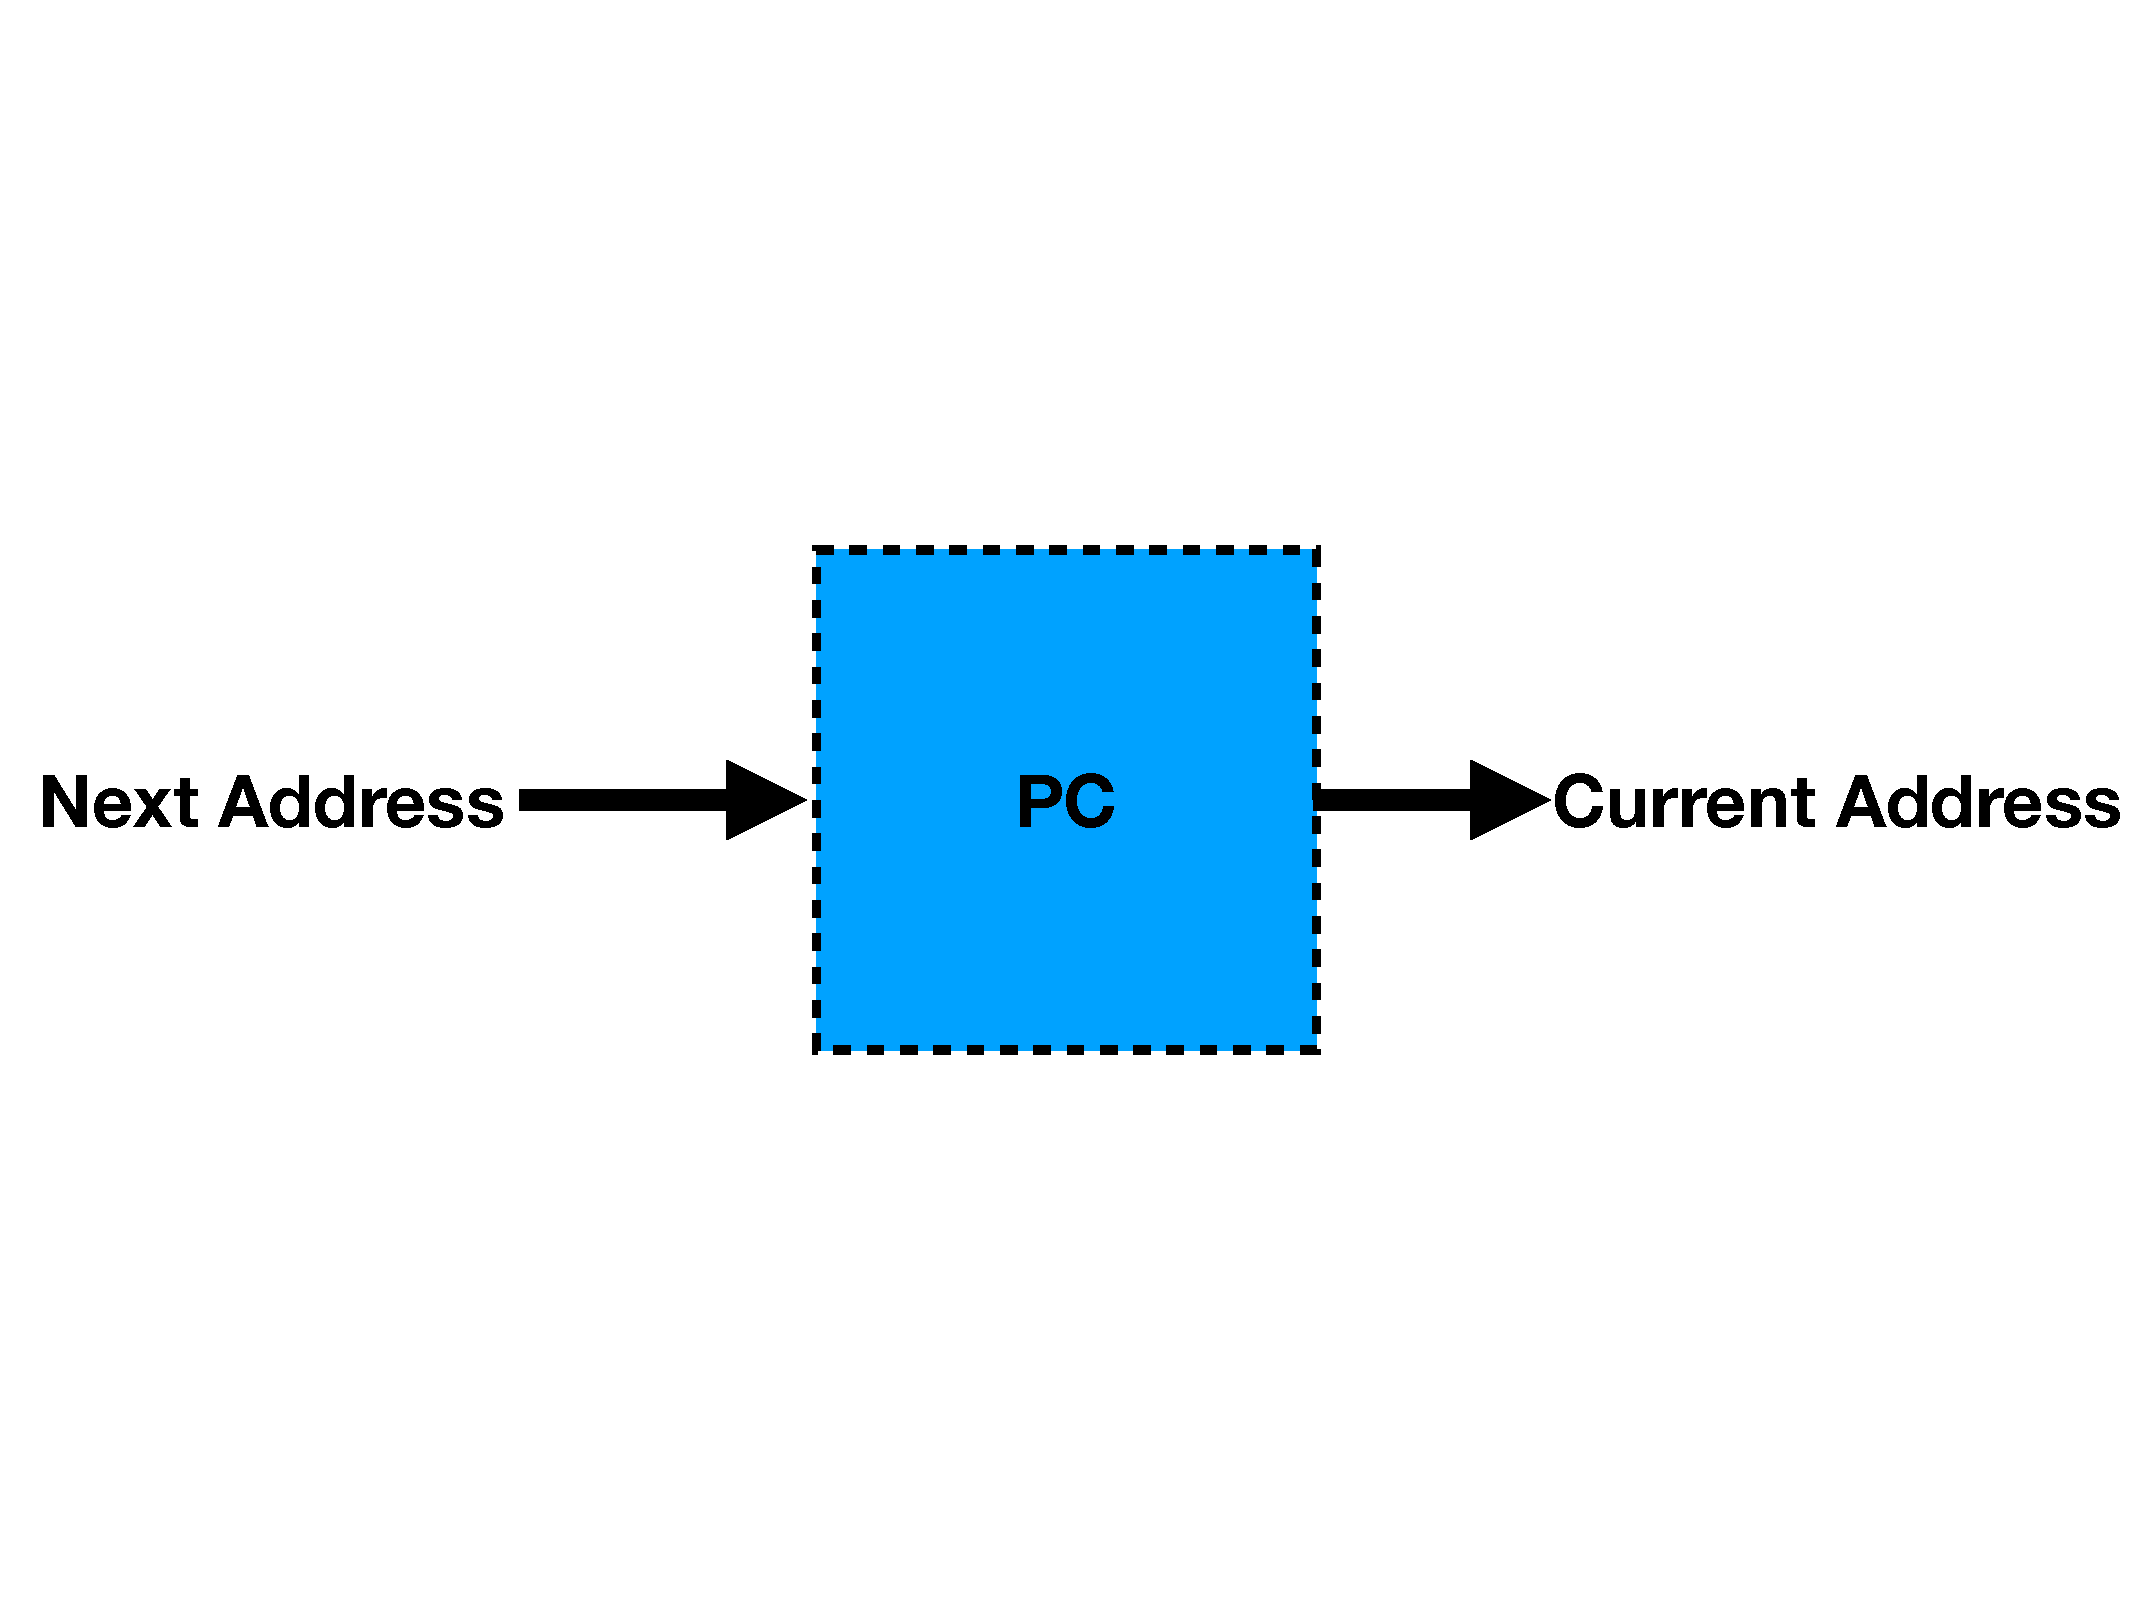
\includegraphics[scale=0.25]{pictures/PC.pdf}
            \caption{Illustration of the clocked \texttt{program counter} process having the next address as input and current address as output.}
            \label{fig:PC}
        \end{figure}
    
        \begin{minipage}{\linewidth}
            \begin{lstlisting}[language={[Sharp]C}, caption={A slice of the PC unit SME code, which contains variable that holds the input address. On every cycle edge it then holds and outputs the current address.},captionpos=b, label = PCSME]
...
    ulong address_hold;

    protected override void OnTick() {
        address_hold = m_Input.Address;
        Output.Address = address_hold;
    }
            \end{lstlisting}
        \end{minipage}   
    
    \subsection{Instruction Memory}
        The \textit{instruction memory}, IM for short, contains the program to be run on the CPU. To implement the instruction memory we create a SME process. It contains a byte array with the instructions to be run. A byte array was chosen to respect the conventions discussed in \ref{section:datatranserinstructions}. This also has the added benefit of having a built-in C$\scalerel*{\#}{X}$ function to read a binary file, which automatically puts the instructions contained within the file, in the correct array format. 
        
        The instructions can also be hand written when declaring the array. Since an instruction is 32-bits, 4 elements in the array are needed to form an instruction, where index 0-3 contains the first instruction.
        
        The instruction memory process has a single input from the program counter, which it uses access the correct instructions. In each cycle we first check whether the address given lies within the instruction array range, if not we shut down the CPU.
        We then construct an instruction, using methods discussed in \ref{section:Operators}, to a temporary variable.
        
        The register fields are then sliced out of this variable and put in the corresponding output buses, \texttt{Read RS1, RS2} and \texttt{Write RS}. The full instruction is also outputted to its own bus, \texttt{instruction}. Lastly we tell the simulation process to keep the CPU running by asserting the \texttt{CPU} bus. The instruction memory process has been illustrated in Figure \ref{fig:IM} and a code segment is shown Listing \ref{IMSME} explaining parts of the code. 
     
        \begin{figure}[h!]
            \centering
            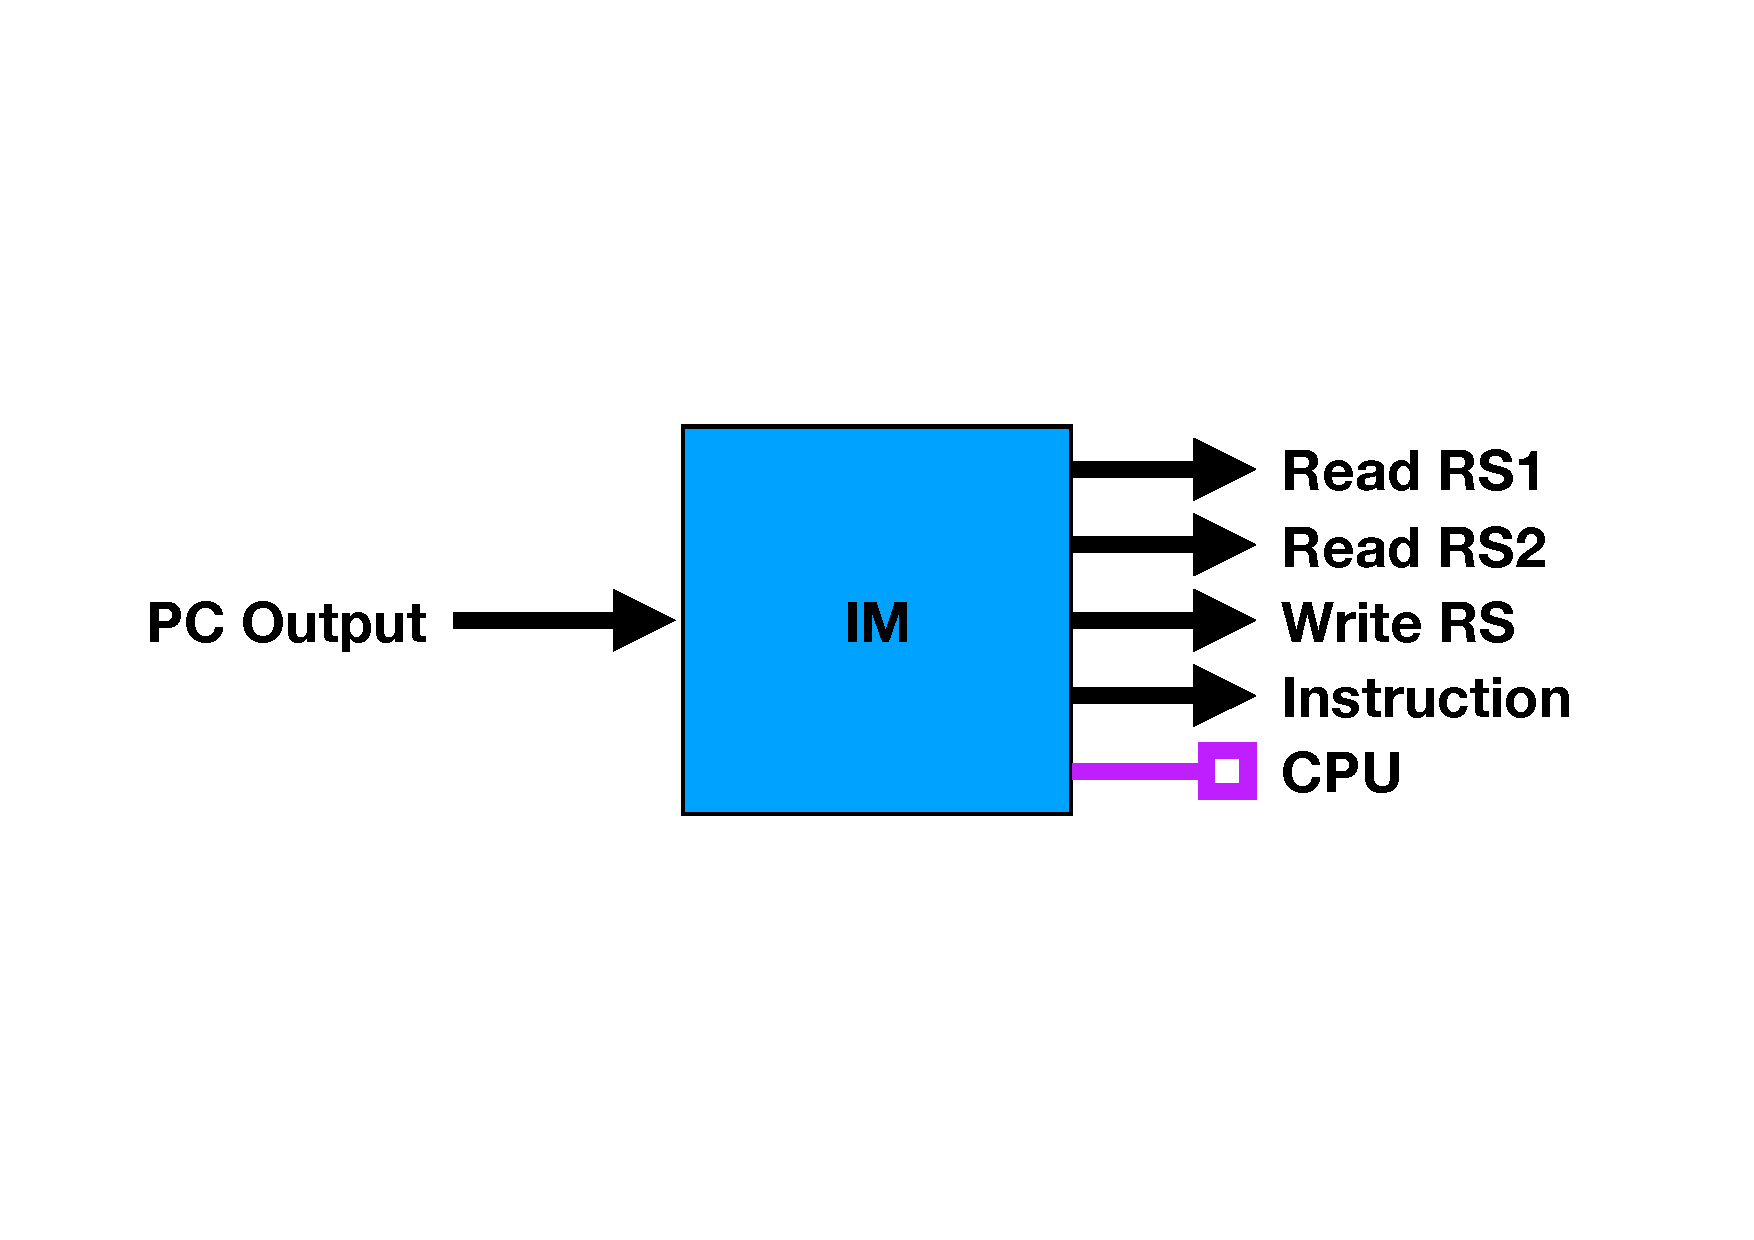
\includegraphics[scale=0.34]{pictures/IM.pdf}
            \caption{Illustration of the \texttt{instruction memory} process, taking the PC output as input and outputting to the 5 buses, \texttt{Read RS1 and RS2}, \texttt{Write RS}, \texttt{Instruction} and \texttt{CPU}.}
            \label{fig:IM}
        \end{figure}
    
        \begin{minipage}{\linewidth}
            \begin{lstlisting}[language={[Sharp]C}, caption={A slice of the Instruction Memory unit SME code. It contains a single byte array, which holds all the instructions to be run. First we check whether the given address to be accessed lies within instruction array, if not we shut down the CPU. We then use the address to access the correct array elements to create a temporary variable, which contains the instruction, as shown in lines 9-12. Hereafter we slice out the fields in the instruction and place the values in the correct busses. Lastly we tell the simulator to keep the CPU running using the CPU bus.},captionpos=b, label = IMSME]
...
    private readonly byte[] Instruction_Memory = System.IO.File.ReadAllBytes("/Users/danielramyar/Downloads/fibo.bin");
            
    protected override void OnTick() {
        ulong temp_address = m_input.Address;
        uint temp_instruction;
            
        if (temp_address >= 0 && temp_address < (uint)Instruction_Memory.Length) {
            temp_instruction = 0u | (uint)Instruction_Memory[temp_address]     << 24
                                  | (uint)Instruction_Memory[temp_address + 1] << 16
                                  | (uint)Instruction_Memory[temp_address + 2] << 8
                                  | (uint)Instruction_Memory[temp_address + 3];
            
            m_Instruction.Current = temp_instruction;
            m_read_1.Address = (uint)temp_instruction >> 15 & (uint)31; 
            m_read_2.Address = (uint)temp_instruction >> 20 & (uint)31; 
            m_write.Address  = (uint)temp_instruction >> 7  & (uint)31; 
            
            m_CPU.Running = true; // Keep CPU running
        }
        else {
            temp_instruction = 0u; // No Instruction
            ...  // Same as in the if statement
            m_CPU.Running = false; // Turn of cpu no more instructions
    }
            \end{lstlisting}
        \end{minipage}  
        
        
        
    
    \subsection{Next instruction Unit}
        To calculate the address of the next instruction in the queue I have created a unit called \texttt{Next}. This unit is very simple, as its only function is to increment the value found in the PC output bus by 4. We increment by 4, since each instruction is 32 bits long and since our instructions are contained in a byte array, we need to move 4 bytes every time we want to access the following instruction. For example if we are placed at index 0, we would have to go to index 4 to access the next instruction (index 0-3 contains instruction 1 and index 4-7 the next).
        
        The next instruction process has the the output from the program counter as input and sends the incremented address to the \texttt{Next Output} bus. The \texttt{Next} process is illustrated in \ref{fig:NEXT} and a code segment is shown in Listing \ref{NEXTSME}.
        
        \begin{figure}[h!]
            \centering
            \includegraphics[scale=0.34]{pictures/Next.pdf}
            \caption{Illustration of the \texttt{next} process, taking the \texttt{PC output} as input and outputs the next instruction adress to the \texttt{next output} bus.}
            \label{fig:NEXT}
        \end{figure}
    
        \begin{minipage}{\linewidth}
            \begin{lstlisting}[language={[Sharp]C}, caption={A slice of the \texttt{Next} process SME code. Here we declare a temporary varible, which contains the program counter output. We increment the temporary variable by four and place it in the output bus.},captionpos=b, label = NEXTSME]
...
        ulong temp;
        
        protected override void OnTick() {
            temp = m_Input.Address + 4;
            Output.Address = temp;
        }
            \end{lstlisting}
        \end{minipage}  
        
    
    \subsection{Register}
    
    \subsection{Arithmetic Logic Unit (ALU)}
    
    \subsection{Immediate generator}
    
    \subsection{Data Memory}
    \improvement{Need to figure out more sections to explain whole datapath}
    
\section{Designing the Control}
    
\section{Single Cycle RISC-V datapath}

\section{Improving the datapath} \improvement{figure out better naming for sections}

    \subsection{RV64I Base Instructions Support}

    \subsection{Supporting R-Format}
    
    \subsection{Supporting I-Format}
    
    \subsection{Supporting S-Format}
    
    \subsection{Supporting B-Format}
    
    \subsection{Supporting U-Format}
    
    \subsection{Supporting J-Format}
    
\section{Debugging the instructions}

    \subsection{Writing assembly to test instructions}
    
    \subsection{Writing simple C code to run on RISC-V}
    
    
    

    